% LaTeX Article Template
\documentclass[12pt]{article}
%% Other packages
\usepackage{amsmath}
\usepackage{amsthm}
\usepackage{titlesec}
\usepackage{soul}
\usepackage{tikz}
\usepackage{tikz-3dplot}
\usepackage{amssymb}
\usepackage{multicol}
\usepackage{float}
\usepackage{calc}
\usepackage{fancybox}
\usepackage{array}
\usepackage[shortlabels]{enumitem}
\usepackage{framed}
\usepackage{hyperref}
\newcolumntype{L}[1]{>{\raggedright\let\newline\\\arraybackslash\hspace{0pt}}m{#1}}
\newcolumntype{C}[1]{>{\centering\let\newline\\\arraybackslash\hspace{0pt}}m{#1}}
\newcolumntype{R}[1]{>{\raggedleft\let\newline\\\arraybackslash\hspace{0pt}}m{#1}}


%% Margins
\usepackage{geometry}
\geometry{verbose,letterpaper,tmargin=1in,bmargin=1in,lmargin=1in,rmargin=1in}

\newcommand{\menuchoice}[2]{{\ttfamily#1..#2}}
\newcommand{\dotdot}{..}

\usepackage{graphicx}

% Array vertical and horizontal stretch
% \def\arraystretch{1.5}%  1 is the default, change whatever you need
% \setlength{\tabcolsep}{12pt}

%\graphicspath{%
\graphicspath{{./figs/}}

%% Paragraph style settings
\setlength{\parskip}{\medskipamount}
\setlength{\parindent}{0pt}

%% Change itemize bullets
\renewcommand{\labelitemi}{$\bullet$}
\renewcommand{\labelitemii}{$\circ$}
\renewcommand{\labelitemiii}{$\diamond$}
\renewcommand{\labelitemiv}{$\cdot$}

%% Shrink section fonts
\titleformat*{\section}{\large\bf}
\titleformat*{\subsection}{\normalsize\it}
\titleformat*{\subsubsection}{\normalsize\bf}

% %% Compress the spacing around section titles
\titlespacing*{\section}{0pt}{1.5ex}{0.75ex}
\titlespacing*{\subsection}{0pt}{1ex}{0.5ex}
\titlespacing*{\subsubsection}{0pt}{1ex}{0.5ex}

%% amsthm settings
\theoremstyle{definition}
\newtheorem{problem}{Problem}
\newtheorem{example}{Example}
\newtheorem{mydef}{Definition}

%% Answer box macros
%% \answerbox{alignment}{width}{height}
\newcommand{\answerbox}[3]{%
  \fbox{%
    \begin{minipage}[#1]{#2}
      \hfill\vspace{#3}
    \end{minipage}
  }
}

%% \answerboxfull{alignment}{height}
\newcommand{\answerboxfull}[2]{%
  \answerbox{#1}{\textwidth}{#2} 
}

%% \answerboxone{alignment}{height} -- for first-level bullet
\newcommand{\answerboxone}[2]{%
  \answerbox{#1}{6.15in}{#2} 
}

%% \answerboxtwo{alignment}{height} -- for second-level bullet
\newcommand{\answerboxtwo}[2]{%
  \answerbox{#1}{5.8in}{#2}
}

%% \graphbox{xmin}{xmax}{ymin}{ymax}{scale}
\newcommand{\graphbox}[5]%[-5, 5, -5, 5, 0.33]
{
\begin{tikzpicture}
     [>=latex,scale=#5]
     
     % Coordinate axes
     \draw [->,very thick] (#1, 0) -- (#2, 0) node[right] {$x$};
     \draw [->,very thick] (0, #3) -- (0, #4) node[above] {$y$};
     
     % Grid
     \draw[step=1cm,thick,dotted] (#1,#3) grid (#2,#4);
   \end{tikzpicture}
   }


%% Redefine maketitle
\makeatletter
\renewcommand{\maketitle}{
  \noindent SA403 -- Networks \\

  \begin{center}\Large{\textbf{\@title}}\end{center}
}
\makeatother

% Set the beginning of a LaTeX document
\begin{document}

%\graphbox{-10}{3}{-5}{10}

\title{Lesson 4: Maximum-flow Problems}

%\graphbox[10][10]

\maketitle


\section*{Notes}

Book acknowledgment:
\section*{Goals}
\begin{itemize}
\item Maximum Flow
\end{itemize}

\section{Try it on your own}

For the following network, the arc labels refer to the maximum allowable (capacity) flow on that arc. Given these capacities, determine the maximum amount of flow $f$ that can be sent from $1$ to $5$.



\begin{center}
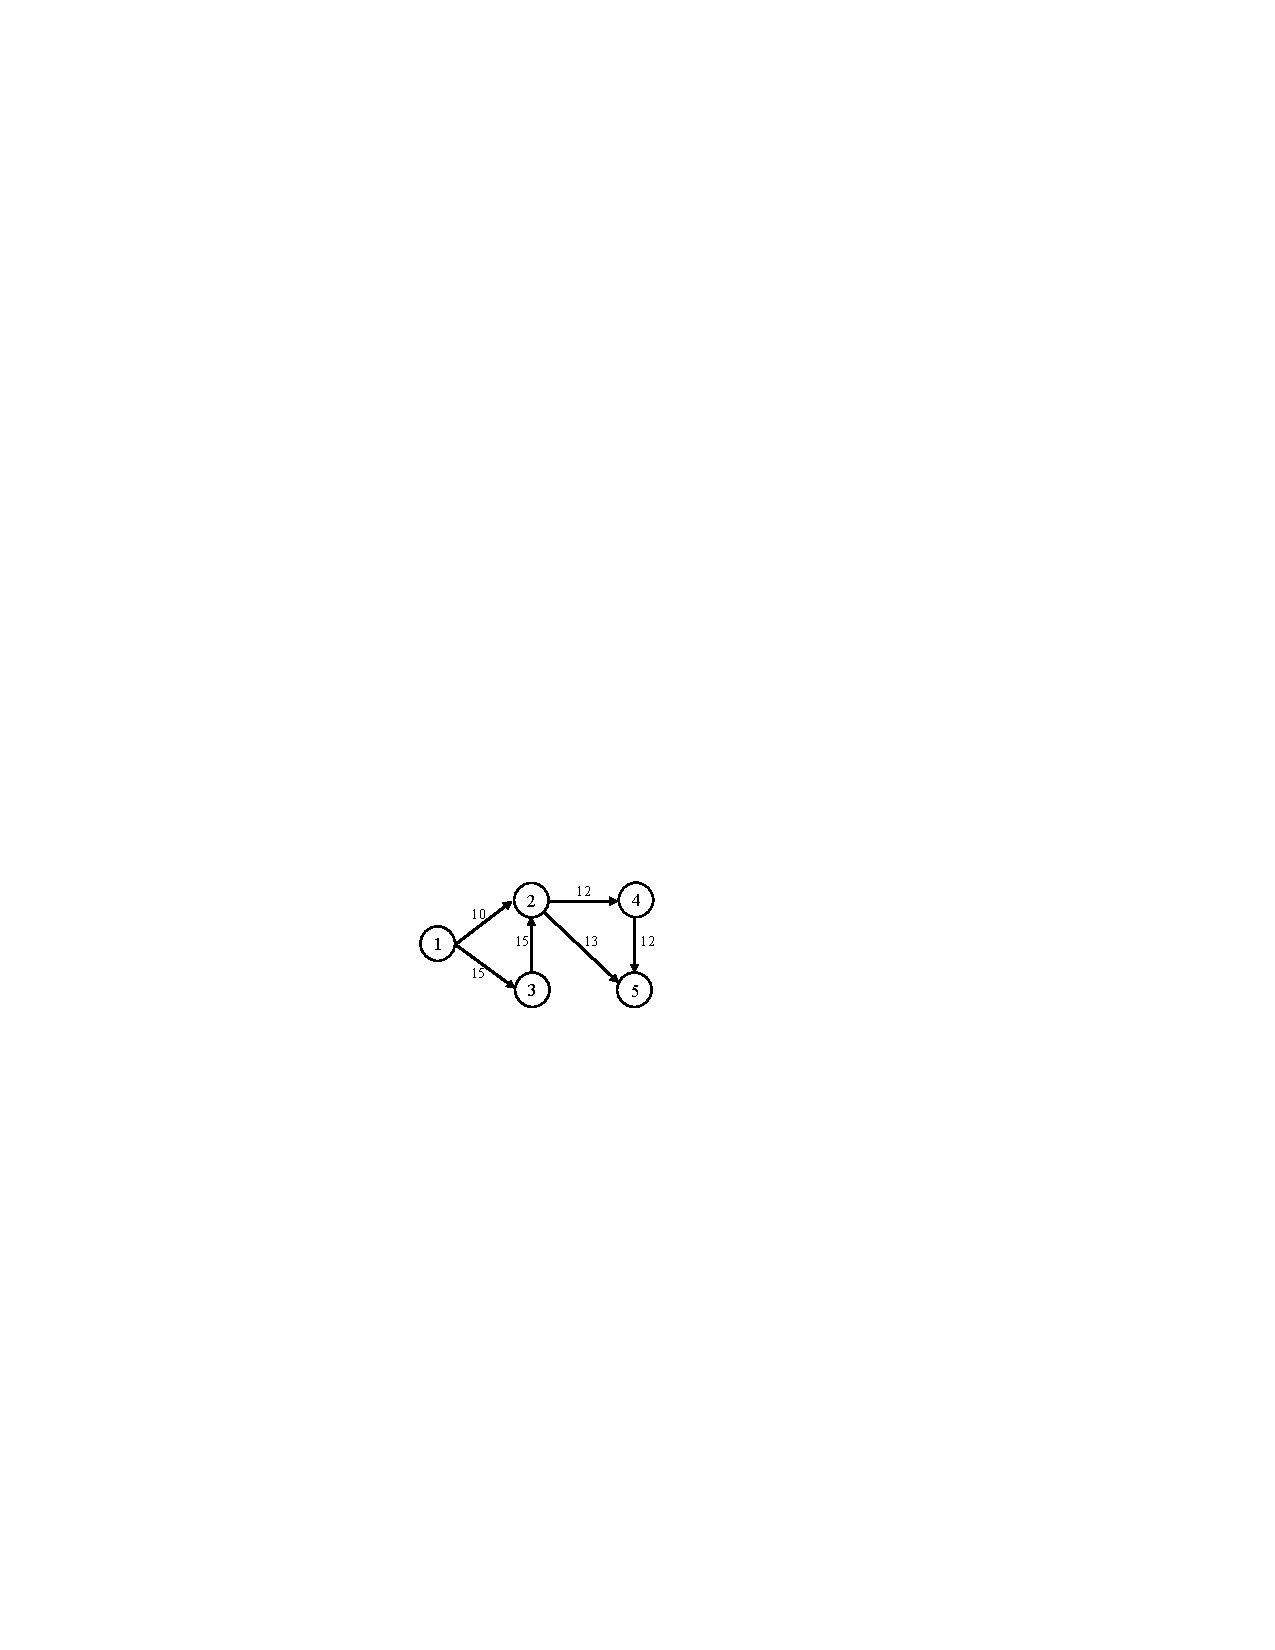
\includegraphics[width=5cm]{shortestpathexample1}
\end{center}
\vfill


How did you go about determining $f$? How could you make your strategy into an algorithm? 

\vfill

\newpage
\section{Problem Definition}

\subsection{Notation}

Given a directed graph $G = (V, A)$, let $c_{uv} \ge 0$ be the capacity on each arc $(u,v) \in A$. For each $(u,v) \in A$, then $(v,u) \notin A$. Determine the maximum amount of flow that can be transmitted from $s$ to $t$ without violating arc capacities or flow conservation among all nodes (incoming flow at each node is equal to the outgoing flow at that node).


\section{Ford-Fulkerson Algorithm}

The Ford-Fulkerson Algorithm is an augmenting-path algorithm that iteratively increases the maximum $s$-$t$ flow $f$ by pushing from $s$ to $t$ on a sequence of arcs having positive residual capacity. A residual graph of a flow network is a graph that indicates additional possible flow given a current set of flows. If there is a path from $s$ to $t$ in the residual network, then additional flow can be sent from $s$ to $t$. Every arc of a residual network has a residual capacity equal to the original capacity of the arc minus the current flow on that arc. 

\textbf{High-level Steps:}


\begin{enumerate}
	\item Set $f = 0$. 
	\item While there is an augmenting $s$-$t$ path in the residual network:
	\begin{itemize}
		\item Add this path-flow to $f$.
	\end{itemize}
	\item Return $f$.

\end{enumerate}

\textbf{Implementation:}

\begin{enumerate}
	\item Set $f = 0$, $\bar{x}_{ij} = 0, \ \forall (i,j) \in A$, $\bar{c}_{ij} = c_{ij}, \ \forall (i,j) \in A$, and $\bar{c}_{ji} = 0, \ \forall (i,j) \in A$. If $\bar{c}_{ij} > 0$, then $(i,j)$ is found among those arcs $A'$ in the residual network.
	\item While a positive residual capacity path exists among the arcs in $A'$:
	\begin{enumerate}[a.]
		\item Let $p$ be any positive residual capacity path among those arcs in $A'$. Let $A_p$ contain all arcs on path $p$, and set the flow $f_p = \textrm{min}\{\bar{c}_{ij}: (i,j) \in A_p \}$.
		\item Increase the total flow on each arc $(i,j) \in A_p$ by setting $\bar{x}_{ij} = \bar{x}_{ij} + f_p, \ \forall (i,j) \in A_p \cap (A \cap A')$ and $\bar{x}_{ij} = \bar{x}_{ij} - f_p, \ \forall (j,i) \in A_p \cap (A' \setminus A)$. 
		\item Update residual capacities $\bar{c}_{ij} = \bar{c}_{ij} - f_p, \ \forall (i,j) \in A_p \cap (A \cap A')$ and $\bar{c}_{ij} = \bar{c}_{ij} + f_p, \ \forall (j,i) \in A_p \cap (A' \setminus A)$. 
		\item Update $A'$: For all $(i,j) \in A'$, if $\bar{c}_{ij} = 0$, then remove $(i,j)$ from $A'$.
		\item Set $f = f + f_p$.
	\end{enumerate}		
	\item Return maximum flow $f$. \label{final_step}

\end{enumerate}


\newpage 

Using the Ford-Fulkerson Algorithm, determine the maximum amount of flow $f$ that can be sent from $1$ to $5$.
\begin{center}
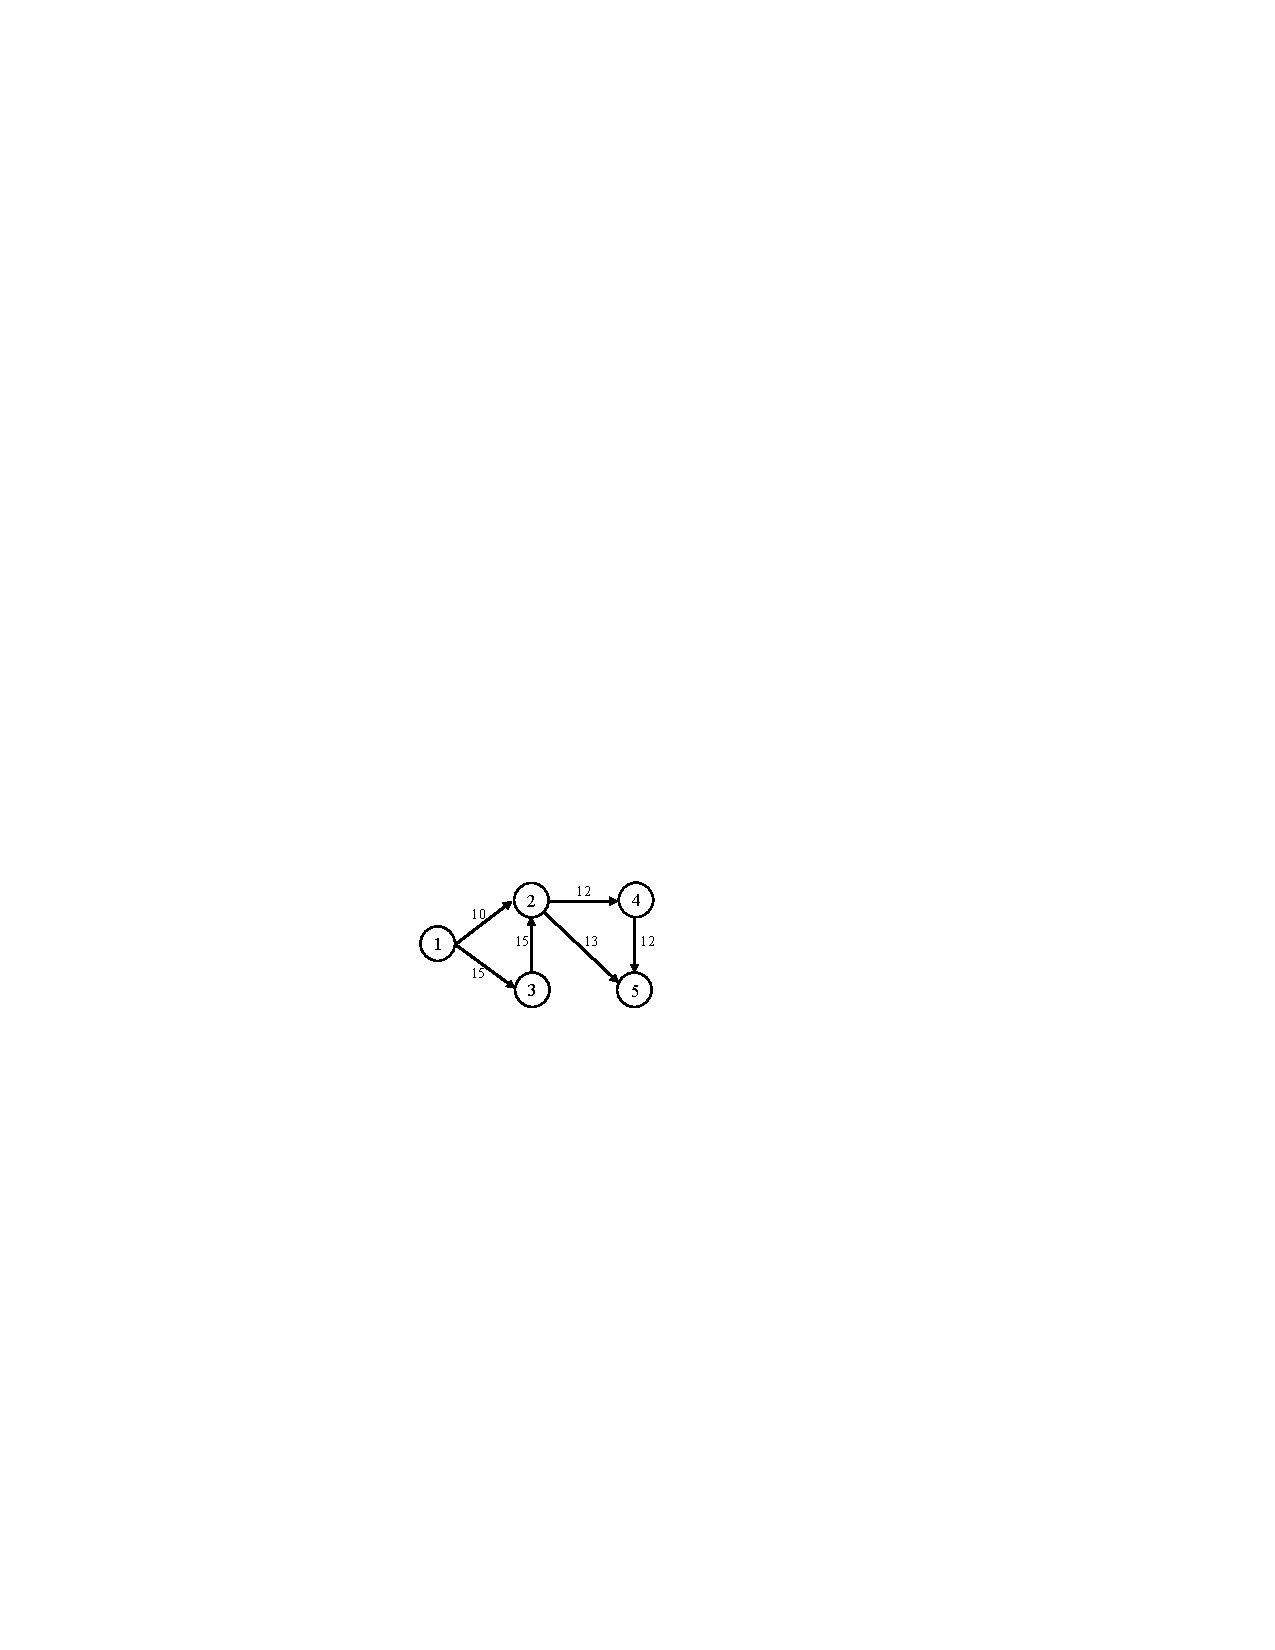
\includegraphics[width=5cm]{shortestpathexample1}
\end{center}
\vfill




\section{Push-relabel Algorithms}

The push-relabel algorithm is generally more efficient than the Ford-Fulkerson Algorithm.  Similar to Ford-Fulkerson, the Push-relable also works on a residual graph. Alternatively, the push-relabel algorithm is drastically different. It works in a decentralized manner. As opposed to examining the entire residual network to find an augmenting path, the P-R algorithm works on one node at a time. During each step of the Ford-Fulkerson, the flow conservation at each node is maintained to be 0. Alternatively, the P-R algorithm allows for the in-flow at each node to exceed the out-flow at that node before reaching the final flow. At termination, though, flow conservation is conserved. 

\textbf{Notes:}

\begin{itemize}
	\item Each node has an associated height value and excess flow value. 
	\item The height value helps to determine whether a node can send more flow to an adjacent node. The P-R algorithm only allows for a node to send flow to other nodes having lower height values.
	\item The excess flow value is the difference of total in-flow and the total out-flow at each node.
	\item Each arc has an associated flow value and capacity.
\end{itemize}

\textbf{High-level Steps:}

\begin{enumerate}
	\item Initialize the height and flow of every node to be 0. Initialize the height of the source node to be equal to the number of vertices in the network. Initalize the flow on each arc to be 0. For all nodes adjacent to the source, flow and excess flow is equal to the capacity initially.
	\item While a vertex has excess flow:
	\begin{enumerate}[a.]
		\item If there is an adjacent node with a smaller height in the residual graph, push flow from the node to the adjacent node having a smaller height. The amount of flow to push is equal to the minimum between the excess flow at that node and the capacity on that arc.
		\item Otherwise, determine the minimum height adjacent node, and increase that heigh value by one.
	\end{enumerate}
	
\end{enumerate}

\textbf{Implementation Steps:}

\begin{enumerate}
	\item Set $f = 0$, $\bar{x}_{ij} = 0, \ \forall (i,j) \in A$, $\bar{c}_{ij} = c_{ij}, \ \forall (i,j) \in A$, and $\bar{c}_{ji} = 0, \ \forall (i,j) \in A$. If $\bar{c}_{ij} > 0$, then $(i,j)$ exists in $A'$ in the residual network. Set $h_i = 0$ and $e_i = 0, \ \forall i \in V$. Finally, set $h_s = |V|$ and $e_s = \sum_{j:(s,j) \in A}c_{sj}$.
	\item While $e_i > 0$ for some node $i \in V \setminus \{t\}$:
	\begin{enumerate}[a.]
		\item While there exists some node $u$ for which $h_u < h_i$ and $(i,u) \in A'$:
		\begin{enumerate}[i.]
		
			\item If $(i,u) \in A \cap A'$, then increase the flow on $(i,u)$ by setting $\bar{x}_{iu} = \bar{x}_{iu} + \textrm{min}\{e_i, \ \bar{c}_{iu}\}$. Set $\bar{c}_{iu} = \bar{c}_{iu} - \textrm{min}\{e_i, \ \bar{c}_{iu}\}$. Update $A'$
			\item Otherwise, if $(i,u) \in A' \setminus A$, the decrease the flow on $(u,i)$ by setting $\bar{x}_{ui} = \bar{x}_{ui} - \textrm{min}\{e_i, \ \bar{c}_{iu}\}$. Set $\bar{c}_{ui} = \bar{c}_{ui} + \textrm{min}\{e_i, \ \bar{c}_{iu}\}$. Update $A'$.
			\item Set $e_i = e_i - \textrm{min}\{e_i, \ \bar{c}_{iu}\}$ and $e_u = e_u + \textrm{min}\{e_i, \ \bar{c}_{iu}\}$. 
		\end{enumerate}
		\item Determine node $u$ for which $h_u = \textrm{min}\{h_j: (u,j) \in A'\}$.
		\item Set $h_u = h_u + 1$.
	\end{enumerate}
	\item Return maximum flow value $e_t$.
\end{enumerate}
\newpage

Using the Push-Relabel Algorithm, determine the maximum amount of flow $f$ that can be sent from $1$ to $5$.
\begin{center}
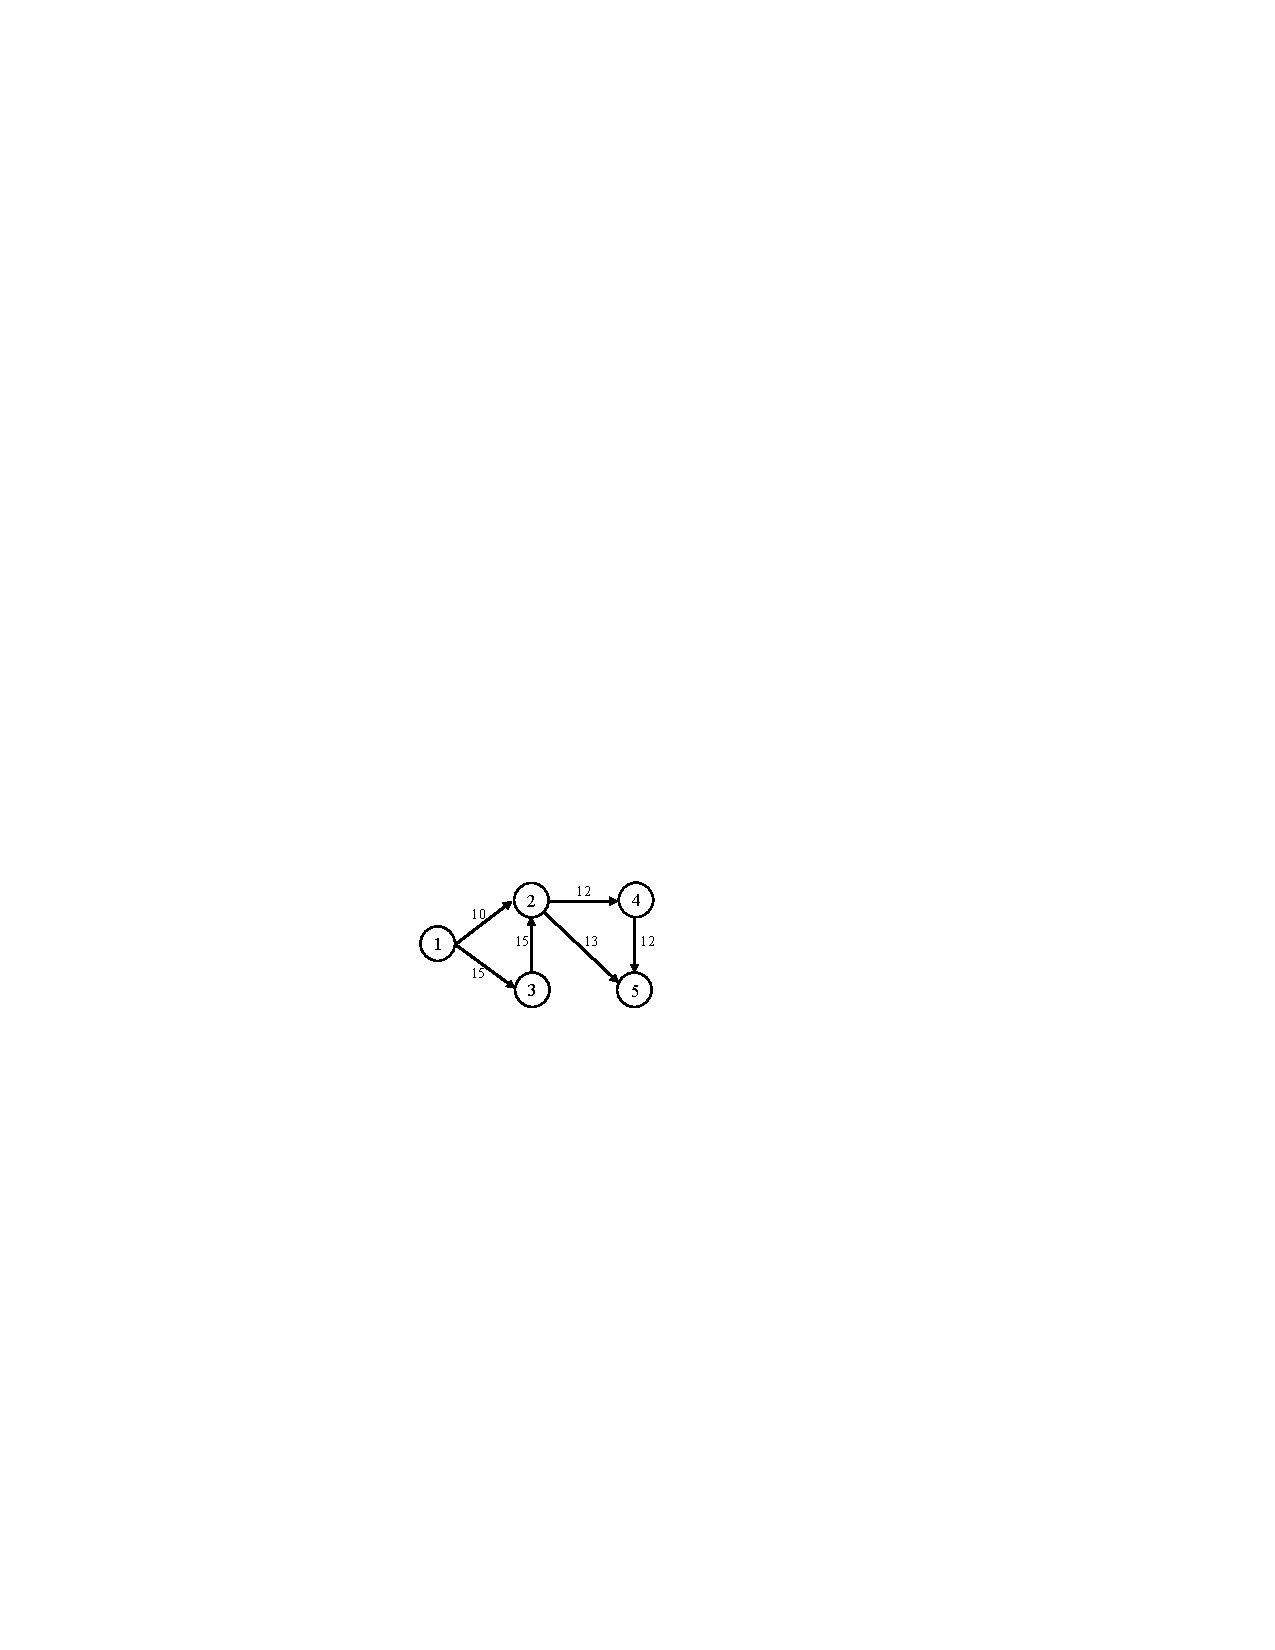
\includegraphics[width=5cm]{shortestpathexample1}
\end{center}
\vfill

\newpage
\section{Ford-Fulkerson vs. Push-Relabel}

\begin{itemize}
	\item What are the similarities between Ford-Fulkerson and the Push-Relabel?
	
	\vfill
	\item What are the differences between Ford-Fulkerson and the Push-Relabel Algorithms?
	\vfill

	\item The P-R algorithm has a running time of $O(V^2E)$ and the Ford-Fulkerson Algorithm has a running time of $O(VE^2)$.
\end{itemize}

\end{document}
